\documentclass[11pt,a4paper]{report}
\usepackage[textwidth=37em,vmargin=30mm]{geometry}
\usepackage{calc,xunicode,amsmath,amssymb,paralist,enumitem,tabu,booktabs,datetime2,xeCJK,xeCJKfntef,listings}
\usepackage{tocloft,fancyhdr,tcolorbox,xcolor,graphicx,eso-pic,xltxtra,xelatexemoji}

\newcommand{\envyear}[0]{2025}
\newcommand{\envdatestr}[0]{2025-02-14}
\newcommand{\envfinaldir}[0]{webdb/2025/20250214/final}

\usepackage[hidelinks]{hyperref}
\hypersetup{
    colorlinks=false,
    pdfpagemode=FullScreen,
    pdftitle={Web Digest - \envdatestr}
}

\setlength{\cftbeforechapskip}{10pt}
\renewcommand{\cftchapfont}{\rmfamily\bfseries\large\raggedright}
\setlength{\cftbeforesecskip}{2pt}
\renewcommand{\cftsecfont}{\sffamily\small\raggedright}

\setdefaultleftmargin{2em}{2em}{1em}{1em}{1em}{1em}

\usepackage{xeCJK,xeCJKfntef}
\xeCJKsetup{PunctStyle=plain,RubberPunctSkip=false,CJKglue=\strut\hskip 0pt plus 0.1em minus 0.05em,CJKecglue=\strut\hskip 0.22em plus 0.2em}
\XeTeXlinebreaklocale "zh"
\XeTeXlinebreakskip = 0pt


\setmainfont{Brygada 1918}
\setromanfont{Brygada 1918}
\setsansfont{IBM Plex Sans}
\setmonofont{JetBrains Mono NL}
\setCJKmainfont{Noto Serif CJK SC}
\setCJKromanfont{Noto Serif CJK SC}
\setCJKsansfont{Noto Sans CJK SC}
\setCJKmonofont{Noto Sans CJK SC}

\setlength{\parindent}{0pt}
\setlength{\parskip}{8pt}
\linespread{1.15}

\lstset{
	basicstyle=\ttfamily\footnotesize,
	numbersep=5pt,
	backgroundcolor=\color{black!5},
	showspaces=false,
	showstringspaces=false,
	showtabs=false,
	tabsize=2,
	captionpos=b,
	breaklines=true,
	breakatwhitespace=true,
	breakautoindent=true,
	linewidth=\textwidth
}






\newcommand{\coverpic}[2]{
    % argv: itemurl, authorname
    Cover photo by #2~~(\href{#1}{#1})
}
\newcommand{\makeheader}[0]{
    \begin{titlepage}
        % \newgeometry{hmargin=15mm,tmargin=21mm,bmargin=12mm}
        \begin{center}
            
            \rmfamily\scshape
            \fontspec{BaskervilleF}
            \fontspec{Old Standard}
            \fontsize{59pt}{70pt}\selectfont
            WEB\hfill DIGEST
            
            \vfill
            % \vskip 30pt
            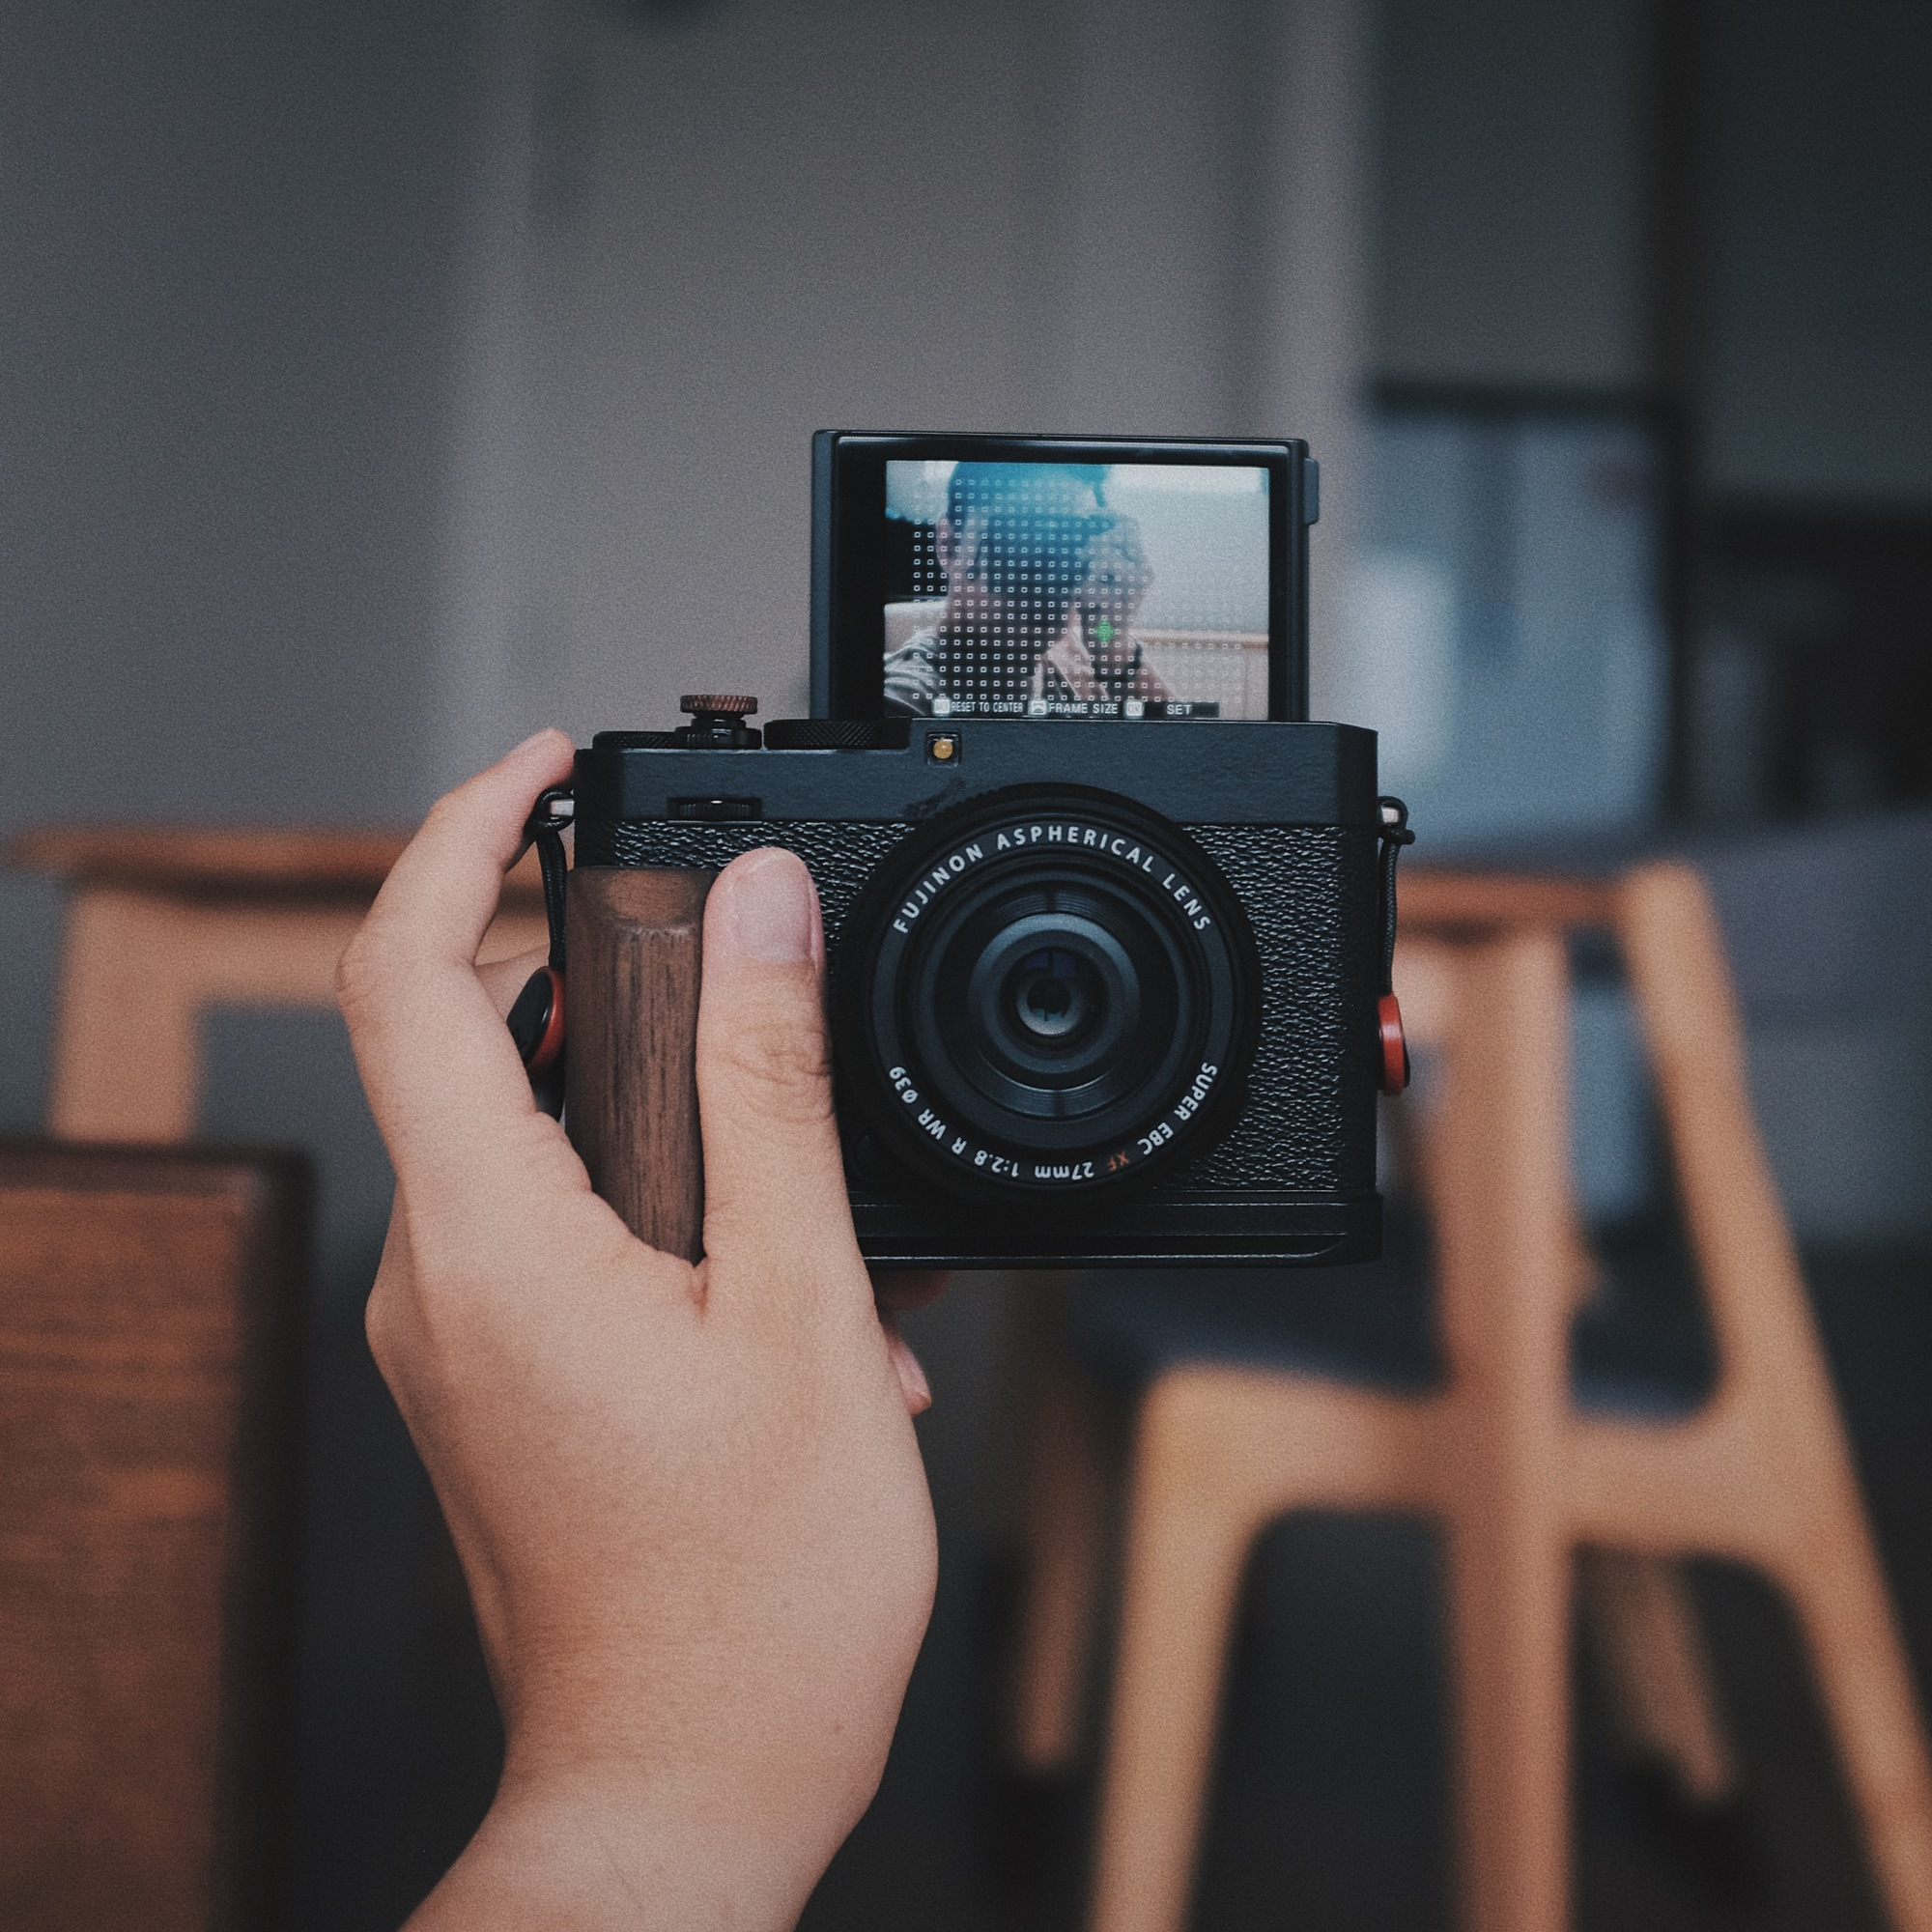
\includegraphics[width=\linewidth]{\envfinaldir/coverpic-prod.jpg}\par
            % \vskip 30pt
            \vfill

            \normalsize\rmfamily\scshape
            \copyright{} The Web Digest Project \hfill\large \envdatestr
        \end{center}
    \end{titlepage}
    % \restoregeometry
}
\newcommand{\simplehref}[1]{%
    \textcolor{blue!80!green}{\href{#1}{#1}}%
}
\renewcommand{\contentsname}{\center\Huge\sffamily\bfseries Contents\par\vskip 20pt}
\newcounter{ipartcounter}
\setcounter{ipartcounter}{0}
\newcommand{\ipart}[1]{
    % \vskip 20pt
    \clearpage
    \stepcounter{ipartcounter}
    \phantomsection
    \addcontentsline{toc}{chapter}{#1}
    % \begin{center}
    %     \Huge
    %     \sffamily\bfseries
    %     #1
    % \end{center}
    % \vskip 20pt plus 7pt
}
\newcounter{ichaptercounter}
\setcounter{ichaptercounter}{0}
\newcommand{\ichapter}[1]{
    % \vskip 20pt
    \clearpage
    \stepcounter{ichaptercounter}
    \phantomsection
    \addcontentsline{toc}{section}{\numberline{\arabic{ichaptercounter}}#1}
    \begin{center}
        \Huge
        \sffamily\bfseries
        #1
    \end{center}
    \vskip 20pt plus 7pt
}
\newcommand{\entrytitlefont}[1]{\subsection*{\raggedright\Large\sffamily\bfseries#1}}
\newcommand{\entryitemGeneric}[2]{
    % argv: title, url
    \parbox{\linewidth}{
        \entrytitlefont{#1}\par\vskip 5pt
        \footnotesize\ttfamily\mdseries
        \simplehref{#2}
    }\vskip 11pt plus 11pt minus 1pt
}
\newcommand{\entryitemGithub}[3]{
    % argv: title, url, desc
    \parbox{\linewidth}{
        \entrytitlefont{#1}\par\vskip 5pt
        \footnotesize\ttfamily\mdseries
        \simplehref{#2}\par\vskip 5pt
        \small\rmfamily\mdseries#3
    }\vskip 11pt plus 11pt minus 1pt
}
\newcommand{\entryitemAp}[3]{
    % argv: title, url, desc
    \parbox{\linewidth}{
        \entrytitlefont{#1}\par\vskip 5pt
        \footnotesize\ttfamily\mdseries
        \simplehref{#2}\par\vskip 5pt
        \small\rmfamily\mdseries#3
    }\vskip 11pt plus 11pt minus 1pt
}
\newcommand{\entryitemHackernews}[3]{
    % argv: title, hnurl, rawurl
    % \parbox{\linewidth}{
    %     \entrytitlefont{#1}\par\vskip 5pt
    %     \footnotesize\ttfamily\mdseries
    %     \simplehref{#3}\par
    %     \textcolor{black!50}{\href{#2}{#2}}
    % }\vskip 11pt plus 11pt minus 1pt
    \begin{minipage}{\linewidth}
            \entrytitlefont{#1}\par\vskip 5pt
            \footnotesize\ttfamily\mdseries
            \simplehref{#3}\par
            \textcolor{black!50}{\href{#2}{#2}}
    \end{minipage}\par\vskip 11pt plus 11pt minus 1pt
}







\begin{document}

\makeheader

\tableofcontents\clearpage




\ipart{Developers}
\ichapter{Hacker News}
\entryitemTwoLinks{Privacy Pass Authentication for Kagi Search}{https://news.ycombinator.com/item?id=43040521}{https://blog.kagi.com/kagi-privacy-pass}

\entryitemTwoLinks{MapTCHA, the open-source CAPTCHA that improves OpenStreetMap [video]}{https://news.ycombinator.com/item?id=43040382}{https://fosdem.org/2025/schedule/event/fosdem-2025-5879-maptcha-the-open-source-captcha-that-improves-openstreetmap/}

\entryitemTwoLinks{'It's a money game to them':son takes on UnitedHealth over elderly father's care}{https://news.ycombinator.com/item?id=43040023}{https://www.theguardian.com/us-news/2025/feb/13/unitedhealth-lawsuit-elderly-patients-care}

\entryitemTwoLinks{Phind 2: AI search with visual answers and multi-step reasoning}{https://news.ycombinator.com/item?id=43039308}{https://www.phind.com/blog/phind-2}

\entryitemTwoLinks{Who exactly needs to get approval from an institutional review board (IRB)?}{https://news.ycombinator.com/item?id=43038395}{https://dynomight.net/irb/}

\entryitemTwoLinks{LibreOffice still kicking at 40, now with browser tricks and real-time collab}{https://news.ycombinator.com/item?id=43038200}{https://www.theregister.com/2025/02/13/libreoffice\_wasm\_zetaoffice/}

\entryitemTwoLinks{Larry Ellison wants to put all America's data in AI, including DNA}{https://news.ycombinator.com/item?id=43038190}{https://www.theregister.com/2025/02/12/larry\_ellison\_wants\_all\_data/}

\entryitemTwoLinks{TSMC faces tough choices amid rumors for Intel foundry collaboration}{https://news.ycombinator.com/item?id=43037668}{https://techsoda.substack.com/p/tsmc-faces-tough-choices-amid-rumors}

\entryitemTwoLinks{White Hat Hackers Expose Iridium Satellite Security Flaws}{https://news.ycombinator.com/item?id=43037623}{https://spectrum.ieee.org/iridium-satellite}

\entryitemTwoLinks{I built a failed startups goods website and named it VcSubsidized.com}{https://news.ycombinator.com/item?id=43037600}{https://vcsubsidized.com/}

\entryitemTwoLinks{DOGE Has Started Gutting a Key US Technology Agency}{https://news.ycombinator.com/item?id=43037426}{https://www.wired.com/story/doge-tts-fired/}

\entryitemTwoLinks{Court Documents Shed New Light on DOGE Activity at Treasury Department}{https://news.ycombinator.com/item?id=43036934}{https://www.zetter-zeroday.com/court-documents-shed-new-light-on-doge-access-and-activity-at-treasury-department/}

\entryitemTwoLinks{Resigning as Asahi Linux project lead}{https://news.ycombinator.com/item?id=43036904}{https://marcan.st/2025/02/resigning-as-asahi-linux-project-lead/}

\entryitemTwoLinks{Better text rendering in Chromium-based browsers on Windows}{https://news.ycombinator.com/item?id=43036593}{https://developer.chrome.com/blog/better-text-rendering-in-chromium-based-browsers-on-windows}

\entryitemTwoLinks{U.K. demand for a back door to Apple data threatens Americans, lawmakers say}{https://news.ycombinator.com/item?id=43036434}{https://www.washingtonpost.com/technology/2025/02/13/apple-uk-security-back-door-adp/}

\entryitemTwoLinks{DOGE staffer is trying to reroute FEMA funds}{https://news.ycombinator.com/item?id=43036042}{https://www.dropsitenews.com/p/doge-fema-funding-access-social-security-numbers}

\entryitemTwoLinks{DOGE as a National Cyberattack}{https://news.ycombinator.com/item?id=43035977}{https://www.schneier.com/blog/archives/2025/02/doge-as-a-national.html}

\entryitemTwoLinks{Cheap blood test detects pancreatic cancer before it spreads}{https://news.ycombinator.com/item?id=43035147}{https://www.nature.com/articles/d41586-025-00438-z}

\entryitemTwoLinks{Reassessing Wayland}{https://news.ycombinator.com/item?id=43034440}{https://dudemanguy.github.io/blog/posts/2025-02-03-wayland-xorg-2/wayland-xorg-2.html}

\entryitemTwoLinks{Self hosted FLOSS fitness/workout tracker}{https://news.ycombinator.com/item?id=43034329}{https://github.com/wger-project/wger}\ichapter{Phoronix}
\entryitemGeneric{\hskip 0pt{}Zed Editor Introduces Open-Source "Zeta" Edit Prediction Model}{https://www.phoronix.com/news/Zed-Zeta-AI-Model-Edit-Predict}

\entryitemGeneric{\hskip 0pt{}Bcachefs Freezes Its On-Disk Format With Future Updates Optional}{https://www.phoronix.com/news/Bcachefs-On-Disk-Format-Freeze}

\entryitemGeneric{\hskip 0pt{}Hector Martin Resigns From The Asahi Linux Project}{https://www.phoronix.com/news/Hector-Martin-Resigns-Asahi}

\entryitemGeneric{\hskip 0pt{}Linux 6.14-rc3 To Fix Platform Profile Support For Newer AMD-Powered ThinkPads}{https://www.phoronix.com/news/Linux-6.14-rc3-Newer-AMD-PP}

\entryitemGeneric{\hskip 0pt{}Google Releases AOM-AV1 3.12 With More Performance Optimizations}{https://www.phoronix.com/news/AOM-AV1-3.12}

\entryitemGeneric{\hskip 0pt{}Wayland Color Management \& HDR Protocol Support Merged}{https://www.phoronix.com/news/Wayland-CM-HDR-Merged}

\entryitemGeneric{\hskip 0pt{}Device Trees For Apple T2 SoCs Slated For Upstreaming In Linux 6.15}{https://www.phoronix.com/news/Linux-6.15-Apple-T2-SoC-DTs}

\entryitemGeneric{\hskip 0pt{}NVIDIA Wiring Up Autonomous Performance Level Selection To Linux CPPC CPUFreq Driver}{https://www.phoronix.com/news/NVIDIA-Auto-Perf-CPPC-CPUFreq}

\entryitemGeneric{\hskip 0pt{}Wayland Color Management \& HDR Protocols Expected To Be Merged Imminently}{https://www.phoronix.com/news/Wayland-Color-HDR-Merging-Soon}\ichapter{Dribbble}
\entryitemGeneric{\hskip 0pt{}Illustration}{https://dribbble.com/shots/25619766-Illustration}

\entryitemGeneric{\hskip 0pt{}Carbon Solutions B2B Dashboard Design}{https://dribbble.com/shots/25554521-Carbon-Solutions-B2B-Dashboard-Design}

\entryitemGeneric{\hskip 0pt{}Love Potion}{https://dribbble.com/shots/25619714-Love-Potion}

\entryitemGeneric{\hskip 0pt{}Pirate Parrot}{https://dribbble.com/shots/25619077-Pirate-Parrot}

\entryitemGeneric{\hskip 0pt{}SPROXX - LOGO DESIGN}{https://dribbble.com/shots/25619328-SPROXX-LOGO-DESIGN}

\entryitemGeneric{\hskip 0pt{}Black Cat Speed Shop®}{https://dribbble.com/shots/25614666-Black-Cat-Speed-Shop}

\entryitemGeneric{\hskip 0pt{}Fintech icons pack download}{https://dribbble.com/shots/25607159-Fintech-icons-pack-download}

\entryitemGeneric{\hskip 0pt{}Self Love}{https://dribbble.com/shots/25607914-Self-Love}

\entryitemGeneric{\hskip 0pt{}Urban Echo}{https://dribbble.com/shots/25608526-Urban-Echo}

\entryitemGeneric{\hskip 0pt{}Cloaked Wireless Device}{https://dribbble.com/shots/25403560-Cloaked-Wireless-Device}

\entryitemGeneric{\hskip 0pt{}Logo tip 001. Symmetry and asymmetry}{https://dribbble.com/shots/25606111-Logo-tip-001-Symmetry-and-asymmetry}

\entryitemGeneric{\hskip 0pt{}World Peace}{https://dribbble.com/shots/25609765-World-Peace}

\entryitemGeneric{\hskip 0pt{}Sentinal - Logo Design}{https://dribbble.com/shots/25606497-Sentinal-Logo-Design}

\entryitemGeneric{\hskip 0pt{}Tanuki}{https://dribbble.com/shots/25606258-Tanuki}

\entryitemGeneric{\hskip 0pt{}Dirty Dutch - Brand Mark / Logo}{https://dribbble.com/shots/25604523-Dirty-Dutch-Brand-Mark-Logo}

\entryitemGeneric{\hskip 0pt{}Cast AI Logo Redesign}{https://dribbble.com/shots/25607135-Cast-AI-Logo-Redesign}

\entryitemGeneric{\hskip 0pt{}Barbershop POS app for booking and payments}{https://dribbble.com/shots/25596116-Barbershop-POS-app-for-booking-and-payments}

\entryitemGeneric{\hskip 0pt{}Seam Logo Redesigned}{https://dribbble.com/shots/25595119-Seam-Logo-Redesigned}

\entryitemGeneric{\hskip 0pt{}HugNecks®}{https://dribbble.com/shots/25596356-HugNecks}

\entryitemGeneric{\hskip 0pt{}Payoneer App Concept Design}{https://dribbble.com/shots/25593820-Payoneer-App-Concept-Design}

\entryitemGeneric{\hskip 0pt{}Nimmio}{https://dribbble.com/shots/25594035-Nimmio}

\entryitemGeneric{\hskip 0pt{}Playtech Animated Icons - Payments}{https://dribbble.com/shots/25592523-Playtech-Animated-Icons-Payments}

\entryitemGeneric{\hskip 0pt{}Aphmau Cat}{https://dribbble.com/shots/25593493-Aphmau-Cat}

\entryitemGeneric{\hskip 0pt{}Design tools}{https://dribbble.com/shots/25592155-Design-tools}


\ipart{Developers~~~~(zh-Hans)}
\ichapter{Solidot}
\entryitemGeneric{\hskip 0pt{}丰田等多家日企内部禁用 DeepSeek}{https://www.solidot.org/story?sid=80549}

\entryitemGeneric{\hskip 0pt{}科学家探测到迄今最高能的中微子}{https://www.solidot.org/story?sid=80548}

\entryitemGeneric{\hskip 0pt{}大脑中的微塑料是否会伤害你?}{https://www.solidot.org/story?sid=80547}

\entryitemGeneric{\hskip 0pt{}NOAA 公开泰坦号内爆音频}{https://www.solidot.org/story?sid=80546}

\entryitemGeneric{\hskip 0pt{}汤森路透在美国赢得 AI 版权侵犯诉讼}{https://www.solidot.org/story?sid=80545}

\entryitemGeneric{\hskip 0pt{}AI 能复制自己}{https://www.solidot.org/story?sid=80544}

\entryitemGeneric{\hskip 0pt{}Anduril 将从微软接手陆军版 HoloLens 头戴式显示设备}{https://www.solidot.org/story?sid=80543}

\entryitemGeneric{\hskip 0pt{}来自半人马座的物质可能已进入太阳系}{https://www.solidot.org/story?sid=80542}

\entryitemGeneric{\hskip 0pt{}真正的自主 AI 也许即将到来}{https://www.solidot.org/story?sid=80541}

\entryitemGeneric{\hskip 0pt{}苹果与阿里合作为国行 iPhone 提供 AI 功能 }{https://www.solidot.org/story?sid=80540}

\entryitemGeneric{\hskip 0pt{}KDE Plasma 6.3 释出}{https://www.solidot.org/story?sid=80539}

\entryitemGeneric{\hskip 0pt{}YouTube CEO 称多数用户通过电视看 YouTube}{https://www.solidot.org/story?sid=80538}

\entryitemGeneric{\hskip 0pt{}Google Chrome 将自动替换泄露的密码}{https://www.solidot.org/story?sid=80537}

\entryitemGeneric{\hskip 0pt{}Kickstarter 将就失败的项目警告用户}{https://www.solidot.org/story?sid=80536}

\entryitemGeneric{\hskip 0pt{}Tumblr 将在后端迁移到 WordPress 后加入联邦宇宙}{https://www.solidot.org/story?sid=80535}

\entryitemGeneric{\hskip 0pt{}比亚迪为低端车型配备天神之眼}{https://www.solidot.org/story?sid=80534}

\entryitemGeneric{\hskip 0pt{}CEO 称 OpenAI 不出售}{https://www.solidot.org/story?sid=80533}

\entryitemGeneric{\hskip 0pt{}苹果释出紧急更新修复 0day}{https://www.solidot.org/story?sid=80532}

\entryitemGeneric{\hskip 0pt{}DeepSeek AI 训练成本并不低}{https://www.solidot.org/story?sid=80531}

\entryitemGeneric{\hskip 0pt{}上海自研 GLP-1 糖尿病新药批准上市}{https://www.solidot.org/story?sid=80530}\ichapter{V2EX}
\entryitemGeneric{\hskip 0pt{}[Android] hyperos 更新 2.0 后,桌面布局只能 4*7 不能 4*6 了,好不习惯,有解吗?}{https://www.v2ex.com/t/1111338}

\entryitemGeneric{\hskip 0pt{}[问与答] 求推荐:类似于闪念贝壳的语音笔记 APP,可以快速通过 apple watch 录音+自动转文本的。}{https://www.v2ex.com/t/1111337}

\entryitemGeneric{\hskip 0pt{}[酷工作] web2 太卷想看看 web3 的看过来, 实习/兼职/全职}{https://www.v2ex.com/t/1111336}

\entryitemGeneric{\hskip 0pt{}[酷工作] 招远程全职后端:主要负责网络安全攻防;也要做开发( PHP ),月薪 3500 美金+技术分红}{https://www.v2ex.com/t/1111334}

\entryitemGeneric{\hskip 0pt{}[分享创造] 如何在一天时间内创建一个最快速的贸易站?}{https://www.v2ex.com/t/1111333}

\entryitemGeneric{\hskip 0pt{}[问与答] [Andorid] box for magisk 配置求助}{https://www.v2ex.com/t/1111332}

\entryitemGeneric{\hskip 0pt{}[酷工作] [全职招聘-菊厂] 研发类岗位 月薪 9k-29k}{https://www.v2ex.com/t/1111331}

\entryitemGeneric{\hskip 0pt{}[宽带症候群] 移动好像解封了部分 cf 的干扰}{https://www.v2ex.com/t/1111330}

\entryitemGeneric{\hskip 0pt{}[问与答] 火绒问题}{https://www.v2ex.com/t/1111329}

\entryitemGeneric{\hskip 0pt{}[OpenAI] openai 放大招了吗}{https://www.v2ex.com/t/1111328}

\entryitemGeneric{\hskip 0pt{}[Android] 出 HP Elite Dragonfly Chromebook}{https://www.v2ex.com/t/1111327}

\entryitemGeneric{\hskip 0pt{}[Node.js] 大家正使用哪个 node 版本,会保持用最新版吗?}{https://www.v2ex.com/t/1111326}

\entryitemGeneric{\hskip 0pt{}[问与答] 最近黄金的火热是怎么回事}{https://www.v2ex.com/t/1111325}

\entryitemGeneric{\hskip 0pt{}[推广] FootballBros - Free Online Soccer Game}{https://www.v2ex.com/t/1111324}

\entryitemGeneric{\hskip 0pt{}[生活] 租房炒菜没有天然气,普通电磁炉效果不好,有没有好办法?}{https://www.v2ex.com/t/1111323}

\entryitemGeneric{\hskip 0pt{}[Apple] 关于 Apple 账户转区的询问}{https://www.v2ex.com/t/1111321}

\entryitemGeneric{\hskip 0pt{}[程序员] 内推的时候内推者貌似可以给被内推者写个评价/评语,这个``评语''的官方名称是什么来着}{https://www.v2ex.com/t/1111320}

\entryitemGeneric{\hskip 0pt{}[宽带症候群] 局域网下 iperf3 测试 udp 会丢包,排查不出问题}{https://www.v2ex.com/t/1111319}

\entryitemGeneric{\hskip 0pt{}[Java] SpringBoot 部分 xml 接口报 Invalid bound statement (not found)问题怎么解决?}{https://www.v2ex.com/t/1111318}

\entryitemGeneric{\hskip 0pt{}[硬件] 精粤主板不支持 dc 调速,这个问题是不是没有解决方案了?}{https://www.v2ex.com/t/1111317}

\entryitemGeneric{\hskip 0pt{}[问与答] 求/许愿/求偶 灵魂 partner}{https://www.v2ex.com/t/1111315}

\entryitemGeneric{\hskip 0pt{}[酷工作] 招聘大量 Java 、Android、iOS}{https://www.v2ex.com/t/1111314}

\entryitemGeneric{\hskip 0pt{}[Java] SpringBoot 调用 XML 接口报 Invalid bound statement (not found)问题怎么解决?}{https://www.v2ex.com/t/1111313}

\entryitemGeneric{\hskip 0pt{}[问与答] 哪吒 2 版权 50 年, 2075 年才能合法免费观看,惊不惊喜意不意外}{https://www.v2ex.com/t/1111312}

\entryitemGeneric{\hskip 0pt{}[问与答] 小说,散文润色 AI 推荐}{https://www.v2ex.com/t/1111311}

\entryitemGeneric{\hskip 0pt{}[路由器] 请问现在有没有支持 esim 的软路由产品,如果现在没有,那将来什么时候会有}{https://www.v2ex.com/t/1111310}

\entryitemGeneric{\hskip 0pt{}[Apple] Mac Mini M4 有必要买 649 延保吗}{https://www.v2ex.com/t/1111308}

\entryitemGeneric{\hskip 0pt{}[问与答] 6 月底 7 月 打算带孩子们去日本,请问如何去比较划算!}{https://www.v2ex.com/t/1111306}

\entryitemGeneric{\hskip 0pt{}[问与答] 为什么美团一类的 O2O 应用在线下核销时要用二维码扫码这种形式?}{https://www.v2ex.com/t/1111305}

\entryitemGeneric{\hskip 0pt{}[问与答] 稳定的 all in one 的 AI 的 API 有推荐的吗?}{https://www.v2ex.com/t/1111303}

\entryitemGeneric{\hskip 0pt{}[问与答] 求教个汉字转统一码的问题}{https://www.v2ex.com/t/1111300}

\entryitemGeneric{\hskip 0pt{}[酷工作] ReactNative 找工作:目标深圳}{https://www.v2ex.com/t/1111298}

\entryitemGeneric{\hskip 0pt{}[Apple] 做了一个文本直接生成流程图的 App,欢迎大家来试用,多多提意见更好!}{https://www.v2ex.com/t/1111297}

\entryitemGeneric{\hskip 0pt{}[问与答] 新手想捐一个馒头的 vip,能不能终身解决下载问题}{https://www.v2ex.com/t/1111296}

\entryitemGeneric{\hskip 0pt{}[问与答] 学习机,值得买给小孩吗?}{https://www.v2ex.com/t/1111293}

\entryitemGeneric{\hskip 0pt{}[酷工作] [全职招聘-上海] Narya.ai | 大模型应用赛道 | 急招 iOS 开发 | 月薪 35~ 55K+ RMB}{https://www.v2ex.com/t/1111292}

\entryitemGeneric{\hskip 0pt{}[问与答] 豆包 app 怎么样才能不让回答里出现抖音短视频}{https://www.v2ex.com/t/1111291}

\entryitemGeneric{\hskip 0pt{}[设计] 时间感知工具,专业工作者必备!正式公测,一年专业版派送中~}{https://www.v2ex.com/t/1111289}

\entryitemGeneric{\hskip 0pt{}[职场话题] 抖音这个开发应该财务自由了吧?抖音工程的 0.8\%代码也是海量吧?欺负外行不懂吗?}{https://www.v2ex.com/t/1111288}

\entryitemGeneric{\hskip 0pt{}[问与答] 非码农,纯好奇云游戏得搞多少台服务器?求大佬科普}{https://www.v2ex.com/t/1111287}

\entryitemGeneric{\hskip 0pt{}[问与答] 在这个论坛混的大多都是程序员吧。。大家觉得继续卷技术还有前途吗?}{https://www.v2ex.com/t/1111286}

\entryitemGeneric{\hskip 0pt{}[问与答] Oliveira 也退役了}{https://www.v2ex.com/t/1111283}

\entryitemGeneric{\hskip 0pt{}[香港] 香港把外币人肉背回来多少限额}{https://www.v2ex.com/t/1111282}

\entryitemGeneric{\hskip 0pt{}[问与答] 手机上还有没有类似和平精英的手游?}{https://www.v2ex.com/t/1111280}

\entryitemGeneric{\hskip 0pt{}[macOS] M4pro 的 mbp 可以装 macos14 吗,有个挺关键的软件只支持到 14 好尴尬}{https://www.v2ex.com/t/1111279}

\entryitemGeneric{\hskip 0pt{}[分享发现] 用 Cursor 做了一个在线计算器网站,欢迎提建议}{https://www.v2ex.com/t/1111276}

\entryitemGeneric{\hskip 0pt{}[问与答] 二线 10k 月薪 996 该去吗?}{https://www.v2ex.com/t/1111275}

\entryitemGeneric{\hskip 0pt{}[程序员] ai 对程序员行业的冲击到底有多大}{https://www.v2ex.com/t/1111274}

\entryitemGeneric{\hskip 0pt{}[酷工作] [深圳][前端][25-50K 19 薪] 京东深圳招人啦}{https://www.v2ex.com/t/1111273}

\entryitemGeneric{\hskip 0pt{}[问与答] 求助各位巨佬,有没有 Web 端解析 PPTX 好的解决方案?}{https://www.v2ex.com/t/1111272}


\ipart{Generic News}







\clearpage
\leavevmode\vfill
\footnotesize

Copyright \copyright{} 2023-2025 Neruthes and other contributors.

This document is published with CC BY-NC-ND 4.0 license.

The entries listed in this newsletter may be copyrighted by their respective creators.

This newsletter is generated by the Web Digest project.

The newsletters are also delivered via Telegram channel \CJKunderline{\href{https://t.me/webdigestchannel}{https://t.me/webdigestchannel}}.\\
RSS feed is available at \CJKunderline{\href{https://webdigest.pages.dev/rss.xml}{https://webdigest.pages.dev/rss.xml}}.

This newsletter is available in PDF at
\CJKunderline{\href{https://webdigest.pages.dev/}{https://webdigest.pages.dev/}}.

The source code being used to generate this newsletter is available at\\
\CJKunderline{\href{https://github.com/neruthes/webdigest}{https://github.com/neruthes/webdigest}}.

This newsletter is also available in
\CJKunderline{\href{http://webdigest.pages.dev/readhtml/\envyear/WebDigest-20250214.html}{HTML}} and
\CJKunderline{\href{https://github.com/neruthes/webdigest/blob/master/markdown/\envyear/WebDigest-20250214.md}{Markdown}}.


\coverpic{https://unsplash.com/photos/a-living-room-with-a-couch-and-a-desk-bqSjAngxOVU}{Laura Cleffmann}


\end{document}
